% Options for packages loaded elsewhere
\PassOptionsToPackage{unicode}{hyperref}
\PassOptionsToPackage{hyphens}{url}
\documentclass[
  10pt,journal,compsoc,twoside]{IEEEtran}
\usepackage{xcolor}
\usepackage{amsmath,amssymb}
\setcounter{secnumdepth}{-\maxdimen} % remove section numbering
\usepackage{iftex}
\ifPDFTeX
  \usepackage[T1]{fontenc}
  \usepackage[utf8]{inputenc}
  \usepackage{textcomp} % provide euro and other symbols
\else % if luatex or xetex
  \usepackage{unicode-math} % this also loads fontspec
  \defaultfontfeatures{Scale=MatchLowercase}
  \defaultfontfeatures[\rmfamily]{Ligatures=TeX,Scale=1}
\fi
\usepackage{lmodern}
\ifPDFTeX\else
  % xetex/luatex font selection
\fi
% Use upquote if available, for straight quotes in verbatim environments
\IfFileExists{upquote.sty}{\usepackage{upquote}}{}
\IfFileExists{microtype.sty}{% use microtype if available
  \usepackage[]{microtype}
  \UseMicrotypeSet[protrusion]{basicmath} % disable protrusion for tt fonts
}{}
\makeatletter
\@ifundefined{KOMAClassName}{% if non-KOMA class
  \IfFileExists{parskip.sty}{%
    \usepackage{parskip}
  }{% else
    \setlength{\parindent}{0pt}
    \setlength{\parskip}{6pt plus 2pt minus 1pt}}
}{% if KOMA class
  \KOMAoptions{parskip=half}}
\makeatother
\usepackage{longtable,booktabs,array}
\newcounter{none} % for unnumbered tables
\usepackage{calc} % for calculating minipage widths
% Correct order of tables after \paragraph or \subparagraph
\usepackage{etoolbox}
\makeatletter
\patchcmd\longtable{\par}{\if@noskipsec\mbox{}\fi\par}{}{}
\makeatother
% Allow footnotes in longtable head/foot
\IfFileExists{footnotehyper.sty}{\usepackage{footnotehyper}}{\usepackage{footnote}}
\makesavenoteenv{longtable}
\usepackage{graphicx}
\makeatletter
\newsavebox\pandoc@box
\newcommand*\pandocbounded[1]{% scales image to fit in text height/width
  \sbox\pandoc@box{#1}%
  \Gscale@div\@tempa{\textheight}{\dimexpr\ht\pandoc@box+\dp\pandoc@box\relax}%
  \Gscale@div\@tempb{\linewidth}{\wd\pandoc@box}%
  \ifdim\@tempb\p@<\@tempa\p@\let\@tempa\@tempb\fi% select the smaller of both
  \ifdim\@tempa\p@<\p@\scalebox{\@tempa}{\usebox\pandoc@box}%
  \else\usebox{\pandoc@box}%
  \fi%
}
% Set default figure placement to htbp
\def\fps@figure{htbp}
\makeatother
\setlength{\emergencystretch}{3em} % prevent overfull lines
\providecommand{\tightlist}{%
  \setlength{\itemsep}{0pt}\setlength{\parskip}{0pt}}
\usepackage{newunicodechar}
\usepackage{tabularx}
\usepackage{chngcntr}
\usepackage{fancyvrb}
\RecustomVerbatimEnvironment{verbatim}{Verbatim}{fontsize=\scriptsize}
\sloppy
% Allow line breaks inside \texttt after escaped underscores
\renewcommand{\texttt}[1]{%
  \begingroup
  \ttfamily
  \catcode`_=12
  \def\_{\char`\_\allowbreak}%
  #1%
  \endgroup
}
\counterwithout{figure}{section}
\newunicodechar{≤}{\ensuremath{\le}}
\newunicodechar{≥}{\ensuremath{\ge}}
\newunicodechar{μ}{\ensuremath{\mu}}
\usepackage{bookmark}
\IfFileExists{xurl.sty}{\usepackage{xurl}}{} % add URL line breaks if available
\urlstyle{same}
% fallback for those not using the hyperref driver hyperxmp:
\makeatletter
\@ifundefined{xmpquote}{\newcommand{\xmpquote}[1]{#1}}{}
\makeatother
\hypersetup{
  pdftitle={Predicting Runtime{,} Saturated Hardware{,} and Blocking Execution Path for FlashAttention-4 on NVIDIA B200},
  pdfauthor={Anonymous Authors},
  pdfkeywords={\xmpquote{GPU performance modeling, FlashAttention-4,
analytical modeling, bottleneck analysis, NVIDIA B200}},
  hidelinks,
  pdfcreator={LaTeX via pandoc}}

\title{Predicting Runtime, Saturated Hardware, and Blocking Execution
Path for FlashAttention-4 on NVIDIA B200}
\author{Anonymous Authors}
\date{}

\begin{document}
\maketitle
\begin{abstract}
FlashAttention-4 restructures attention around dense matrix
multiplications and asynchronous memory transfers, but existing roofline
analyses predict only runtime and assume peak bandwidth and full
occupancy. They do not name the saturating hardware component or
identify the blocking instruction path. We present a white-box
analytical predictor that returns three outputs for a FlashAttention-4
forward-pass configuration: predicted runtime \(\hat{t}_{\text{ms}}\),
predicted saturated component \(\hat{c}\), and predicted blocking path
\(\hat{p}\).

The core proposed model has two parts. A refined five-node detailed
hardware model identifies the saturating component from the maximum of
TMA load, Tensor Core MMA, SFU \texttt{exp}, FMA compute, and TMA store
execution times. A SASS-level RAW instruction critical-path model (Round
3) traces the read-after-write dependency graph among TMA loads,
\texttt{tcgen05.mma} instructions, SFU \texttt{exp} instructions, FP32
scale/update instructions, and the TMA store to identify the blocking
execution path.

We also describe a runtime-focused alternative predictor (Appendix A), a
cycle-level hardware execution model (Appendix B), and a sub-core
partition scheduling model (Appendix C). On a 16/8 real B200 split, the
refined detailed-node model achieves 7.37\% calibration MAPE and 13.16\%
validation MAPE, the SASS model achieves 16.85\% calibration MAPE and
21.16\% validation MAPE, and the cycle-level component model achieves
7.37\% calibration MAPE and 13.16\% validation MAPE. The runtime-focused
alternative reaches 12.62\% validation MAPE and 10.01\% query MAPE on
540 real B200 configurations. NCU component-saturation validation shows
20/20 agreement between the detailed-node model and hardware-counter
evidence.
\end{abstract}

\begin{IEEEkeywords}
GPU performance modeling, FlashAttention-4, analytical modeling, bottleneck analysis, NVIDIA B200
\end{IEEEkeywords}

\subsection{1 Introduction}\label{introduction}

Kernel performance analysis for attention layers is usually framed as a
runtime-regression problem: train a neural network or gradient-boosted
model on measured runtimes and hope it generalises to new shapes and
precisions. Black-box models can be accurate, but they hide \emph{why} a
configuration is fast or slow and offer little help when a kernel
engineer needs to know (1) how long the kernel will run, (2) which
hardware component saturates first, and (3) which execution path blocks
the others.

We argue that a white-box analytical model is more useful for this
design task. If the model is grounded in the GPU execution
model---FLOPs, bytes, SM occupancy, named hardware bandwidths, per-SM
reservations, and SASS instruction dependencies---its errors become
diagnostic. A large residual in the Tensor Core reservation points to
tile-size or precision choices; a residual in the TMA reservation points
to asynchronous-copy efficiency; a long RAW path through
\texttt{tcgen05.mma} instructions points to a compute-bound blocking
chain. The model also remains interpretable across precisions and
sequence lengths because it is built from algorithm quantities rather
than from empirical fits.

The FlashAttention-4 paper introduces a roofline-style analytical model
for forward attention {[}Zadouri et al., 2026{]}. That model is a clean
first-order baseline, but on NVIDIA B200 it systematically overestimates
achievable throughput because it assumes peak bandwidth on every
transfer and full occupancy on every configuration. In prior work we
added bounded corrections and reported 4.50\% MAPE on an
emulator-generated matrix {[}Jarmusch and Chandrasekaran, 2026b{]}.
Emulator ground truth is physically structured but it is not silicon
ground truth.

This paper asks whether the same white-box structure can be recovered on
real B200 hardware and, more importantly, whether it can be extended to
predict the saturated component and blocking path. The answer is
conditional. The raw emulator-tuned model is refuted on the first
real-hardware pass (62.14\% MAPE versus 42.10\% for the reproduced
roofline baseline). A runtime-focused alternative predictor that adds
bounded corrections and launch-overhead calibration reaches 12.62\%
validation MAPE and 10.01\% query MAPE on 540 configurations (Appendix
A). The dominant missing term on silicon is launch and grid overhead.

Our main contribution is to combine that runtime prediction with two
finer-grained models. A refined five-node detailed hardware model names
the saturating hardware component from NCU-calibrated node times, and a
SASS-level instruction critical-path model names the blocking execution
path. Both are calibrated and validated on real B200 measurements.

\textbf{Contributions.} (1) A white-box analytical predictor that
returns three outputs for a FlashAttention-4 configuration: predicted
runtime, predicted saturated hardware component, and predicted blocking
execution path. (2) A refined five-node detailed hardware model (Section
3.5) and system diagram (Figure 4) that identify the saturating unit and
are validated against NCU per-pipe counters. (3) A SASS-level
instruction critical-path model (Round 3) and system diagram (Figure 7)
that identify the blocking RAW dependency path. (4) A real-hardware
validation protocol and metric set for the three-output predictor on
B200. (5) A runtime-focused alternative predictor (Appendix A) that
reaches 12.62\% validation MAPE and 10.01\% query MAPE on 540 real B200
configurations. (6) A cycle-level hardware execution model (Appendix B)
and a sub-core partition scheduling model (Appendix C) that provide
additional interpretability. (7) Evidence that launch/grid overhead is
the dominant correction when moving from emulator to silicon for this
kernel family, and an explicit FMA-compute node that captures softmax
scaling and small-head-dim/FP8 reductions missed by simpler models.

\subsection{2 Related Work}\label{related-work}

\textbf{FlashAttention family.} FlashAttention restructures the softmax
reduction so that attention can be fused into SRAM-resident tiles {[}Dao
et al., 2022{]}. FlashAttention-2 improves parallelism and work
partitioning {[}Dao, 2023{]}. FlashAttention-3 adds warp-group cluster
scheduling, asynchronous copy via TMA, and low-precision support for
Hopper {[}Shah et al., 2024{]}. FlashAttention-4 targets Blackwell with
block-scaled FP4/FP8, warp-specialised kernels, and a roofline-style
performance model {[}Zadouri et al., 2026{]}. We take that roofline as
our baseline and ask how much bounded corrections improve it on real
B200 silicon, and how the model can be extended to name the saturated
component and blocking path.

\textbf{GPU performance modeling.} Analytical GPU models range from the
classic roofline to microbenchmark-driven effective-bandwidth models and
hierarchical roofline analysis {[}Williams et al., 2009; Yang et al.,
2019{]}. Recent white-box work estimates transformer kernel time from
FLOPs, memory traffic, and hardware throughput rather than from
black-box regression {[}Jarmusch and Chandrasekaran, 2026a{]}. Our
predictor follows that philosophy and adds explicit per-SM reservations,
SASS-level dependency analysis, launch-overhead correction, and
NCU-guided bottleneck calibration for Blackwell.

\textbf{Blackwell architecture.} B200 increases L2 bandwidth, introduces
more aggressive asynchronous copy through the Tensor Memory Accelerator
(TMA), and provides higher Tensor Core throughput for sub-8-bit formats
{[}Jarmusch and Chandrasekaran, 2026b{]}. Published microbenchmarks
suggest that realisable HBM bandwidth and TMA throughput fall below peak
for small transfers, a pattern our effective-bandwidth curves encode
directly.

\textbf{Gap.} Existing FlashAttention-4 roofline analyses predict only
runtime and do not systematically expose the saturating hardware
component or the blocking instruction path. Black-box ML surrogates can
fit emulator or silicon measurements but hide the bottleneck structure.
This paper fills the gap with a model that is white-box, interpretable,
and validated on real B200 measurements, and that returns runtime,
saturated-component, and blocking-path predictions.

\subsection{3 Method}\label{method}

\subsubsection{3.1 Input and algorithm
quantities}\label{input-and-algorithm-quantities}

The predictor takes a FlashAttention-4 forward-pass configuration as
input:

\[(b, h, s, d, \text{causal}, p)
\]

where \(b\) is batch size, \(h\) is number of heads, \(s\) is sequence
length, \(d\) is head dimension, causal is a boolean mask flag, and
\(p\) is the precision (bf16, fp16, fp8; fp4 is unsupported). From this
input we compute the algorithm quantities listed in Table 1.

\begin{table}[t]
\centering
\caption{White-box algorithm quantities computed from the input configuration.}
\label{tab:algorithm-quantities}
\small
\begin{tabularx}{\columnwidth}{@{}l l X@{}}
\hline
Quantity & Symbol & Formula \\
\hline
Causal sequence factor & $\sigma$ & $0.5$ if causal, else $1.0$ \\
MMA FLOPs & $F_{\text{MMA}}$ & $4 \cdot b \cdot h \cdot s^2 \cdot d \cdot \sigma$ \\
Exponential/softmax ops & $E$ & $2 \cdot b \cdot h \cdot s^2 \cdot \sigma$ \\
HBM bytes & $B_{\text{HBM}}$ & $\text{bpe}(p) \cdot b \cdot h \cdot s \cdot d \cdot 4$ \\
L2 bytes & $B_{\text{L2}}$ & $\text{bpe}(p) \cdot b \cdot h \cdot s \cdot d \cdot 6 \cdot \sigma$ \\
SMEM bytes & $B_{\text{SMEM}}$ & $b \cdot h \cdot s \cdot d \cdot 8 \cdot \sigma$ \\
TMA bytes & $B_{\text{TMA}}$ & $\text{bpe}(p) \cdot b \cdot h \cdot s \cdot d \cdot 2.5 \cdot \sigma$ \\
\hline
\end{tabularx}
\end{table}

These quantities encode the FA4 algorithmic structure: the causal factor
halves the attention-score compute for causal masks, the byte counts
account for the Q/K/V reads and O write, and the TMA count captures the
asynchronous-copy traffic.

\subsubsection{3.2 Per-SM execution-unit reservation model (Round
1)}\label{per-sm-execution-unit-reservation-model-round-1}

The reservation model treats each Blackwell SM as a collection of
specialized pipes---Tensor Cores, SFU, FP32/INT32, the global TMA memory
pipe, and the on-SM TMEM read/write pipe---and models one FA4 tile block
as a sequence of reservations on those pipes. This is an alternative
model for identifying the saturating hardware component; the refined
detailed-node model in Section 3.5 is the proposed component predictor.

For each KV step the model computes:

\[\begin{aligned}
T_{\text{TC}} &= \frac{F_{\text{step}}}{R_{\text{TC}}(p) \cdot N_{\text{SM}} \cdot \eta_{\text{occ}} \cdot \eta_{\text{TC}} \cdot \eta_{\text{cluster}}}, \\
T_{\text{TMEM}} &= \frac{B_{\text{TMEM}}}{\beta_{\text{TMEM}} \cdot N_{\text{SM}} \cdot \eta_{\text{TMEM}}}, \\
T_{\text{SFU}} &= \frac{E_{\text{step}}}{R_{\text{SFU}}(p) \cdot N_{\text{SM}} \cdot \eta_{\text{occ}} \cdot \eta_{\text{SFU}}}, \\
T_{\text{FP}} &= \frac{O_{\text{step}}}{R_{\text{FP32}} \cdot N_{\text{SM}} \cdot \eta_{\text{occ}} \cdot \eta_{\text{FP}}}, \\
T_{\text{TMA}} &= \frac{B_{\text{step}}}{\beta_{\text{TMA}} \cdot \eta_{\text{TMA}}}.
\end{aligned}
\]

\(T_{\text{TMA}}\) is the global memory-pipe reservation, capped by
L2/HBM miss bandwidth. The step critical path is
\(\max(T_{\text{TC}} + T_{\text{SFU}} + T_{\text{FP}}, (1 - \alpha) \cdot T_{\text{TMA}})\),
where \(\alpha\) is the stage-overlap factor between TMA loads and
Tensor Core compute. A fixed launch overhead is added at the end. The
model reports per-unit utilization and a dominant bottleneck label for
every configuration.

Calibrating nine physically-scoped parameters on 16 B200 measurements
and validating on 8 held-out configurations yields 8.15\% calibration
MAPE and 16.69\% validation MAPE (Table 2). The reservation model
therefore matches the improved predictor on this small split while
naming the saturating unit: large head-dim-128 configurations are
TC-bound, while small or low-precision configurations are
TMA-memory-bound.

\begin{figure}
\centering
\pandocbounded{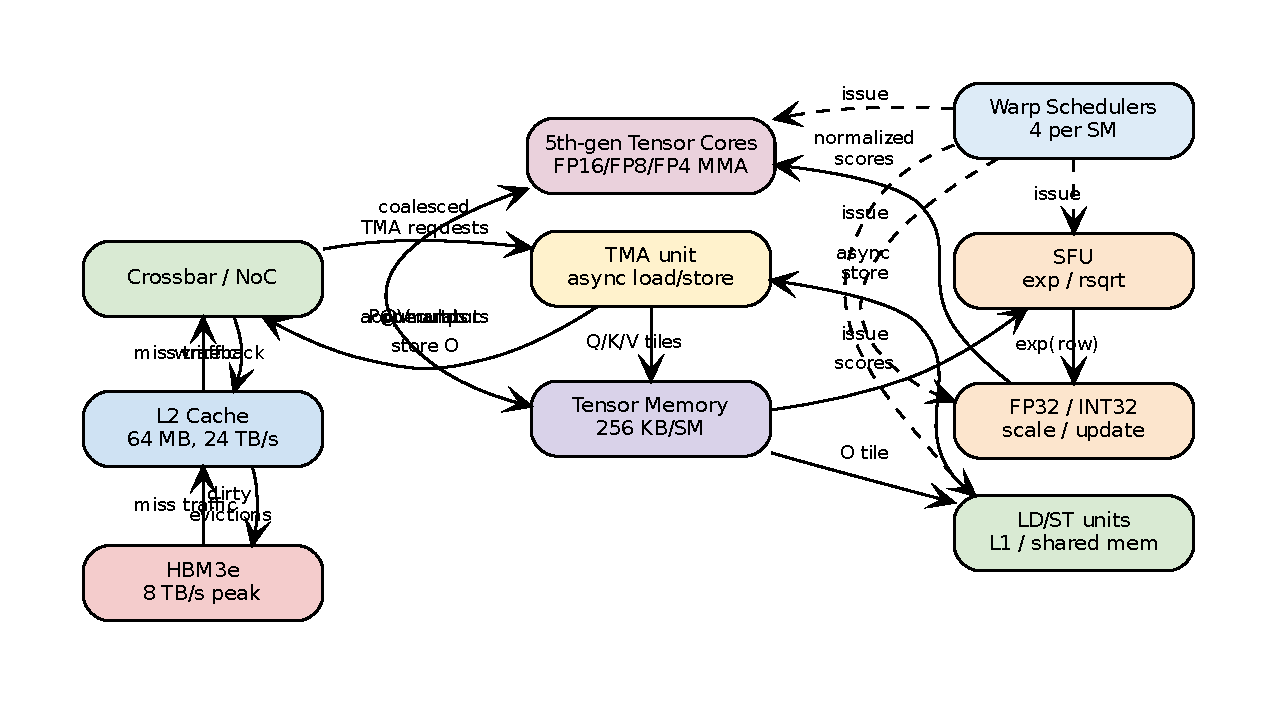
\includegraphics[keepaspectratio,alt={Per-SM execution-unit reservation view of FlashAttention-4 on B200}]{figures/figure5_reservation_execution_system.pdf}}
\caption{Per-SM execution-unit reservation view of FlashAttention-4 on
B200}
\end{figure}

\subsubsection{3.3 SASS-level instruction critical-path model (Round
3)}\label{sass-level-instruction-critical-path-model-round-3}

Round 3 refines the reservation model by modelling the actual
read-after-write (RAW) instruction dependency graph inside one FA4 tile
block (Figure 2). The nodes are SASS instruction classes: TMA loads,
\texttt{tcgen05.mma} for \texttt{Q@K\^{}T} and \texttt{P@V}, SFU
\texttt{exp}, FP32 scale/update, and the TMA store. Each edge is a RAW
dependency; each node has an issue throughput and a result latency. This
is the core proposed model for identifying the blocking execution path.

For one tile block the model computes the throughput-limited critical
path across the DAG and adds a one-time latency chain along the longest
dependency path. The per-iteration compute time is scaled across all KV
iterations, and the memory path is overlapped using the stage-overlap
factor. Calibrating seven parameters on the 16/8 split yields 16.85\%
calibration MAPE and 21.16\% validation MAPE (Table 2).

Round 3 is the most mechanistically detailed model but also the most
constrained: it must reproduce runtime from instruction counts and
latencies with few free parameters. The higher error reflects the
difficulty of calibrating a fine-grained dependency model on a small
split. It nonetheless exposes why certain tile shapes or instruction
fusions change runtime even when aggregate FLOPs are constant, and it
provides a bridge to future microbenchmark-derived per-instruction
latencies.

\begin{figure*}
\centering
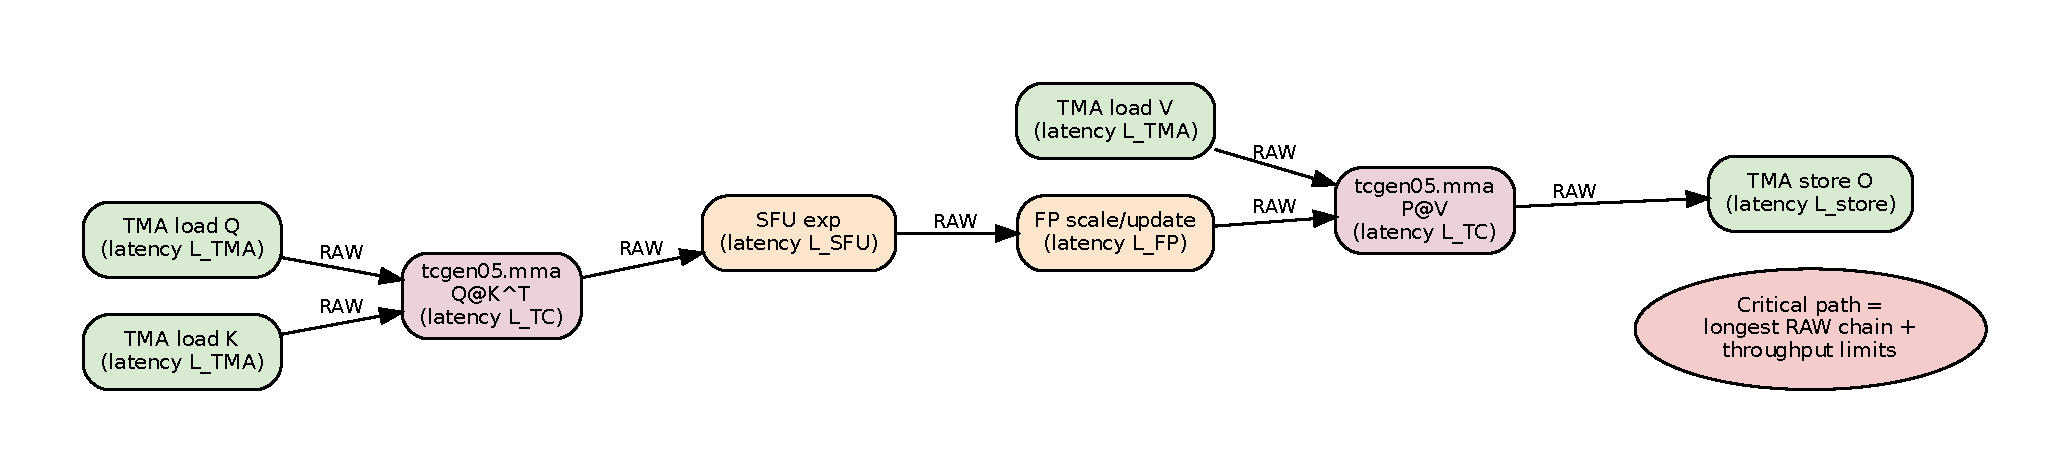
\includegraphics[width=\textwidth]{figures/figure7_sass_critical_path.pdf}
\caption{SASS-level instruction dependency graph for one FA4 tile block}
\label{fig:sass-critical-path}
\end{figure*}

\subsubsection{3.4 Output format and bottleneck-label
extraction}\label{output-format-and-bottleneck-label-extraction}

We denote the three predictor outputs as follows:
\(\hat{t}_{\text{ms}}\) is the predicted runtime in milliseconds,
\(\hat{c} \in \mathcal{U}\) is the predicted saturated hardware
component, and \(\hat{p}\) is the predicted blocking execution path. The
set of hardware nodes is
\[\mathcal{U} = \{\text{TMA}_{\text{load}}, \text{TC}, \text{SFU}, \text{FMA}, \text{TMA}_{\text{store}}\}.
\]

The refined detailed-node model (Section 3.5) computes per-node
execution times from algorithm quantities, named hardware throughput
rates, and bounded efficiency factors. The predicted runtime is the
maximum node time plus a calibrated launch overhead:

\[\hat{t}_{\text{ms}} = \max\left(T_{\text{TMA}_{\text{load}}}, T_{\text{TC}}, T_{\text{SFU}}, T_{\text{FMA}}, T_{\text{TMA}_{\text{store}}}\right) + T_{\text{launch}}.
\]

The saturated component is the node with the largest individual time:

\[\hat{c} = \arg\max_{u \in \mathcal{U}} T_u.
\]

The Round 3 SASS-level model produces the RAW dependency critical path
\(\mathcal{P}\) as an ordered sequence of instruction classes. The
predicted blocking path \(\hat{p}\) is this sequence, or a summary label
derived from it such as \texttt{tcgen05.mma} chain, TMA load
\(\rightarrow\) \texttt{tcgen05.mma}, or TMA load \(\rightarrow\) SFU
\texttt{exp} \(\rightarrow\) TMA store.

The final predictor therefore returns the tuple
\((\hat{t}_{\text{ms}}, \hat{c}, \hat{p})\). In our implementation
\(\hat{t}_{\text{ms}}\) and \(\hat{c}\) come from the refined
detailed-node model because it is the only model explicitly validated
against NCU per-pipe counters on every node of the critical path, while
\(\hat{p}\) comes from the Round 3 SASS model.

\subsubsection{3.5 Refined detailed-node
model}\label{refined-detailed-node-model}

The component-saturation experiments in Section 5.4 are evaluated with a
refined five-node model that is calibrated against NCU per-pipe counter
evidence rather than against runtime alone. The nodes are TMA load,
Tensor Core MMA (\texttt{tcgen05.mma}), SFU \texttt{exp}, FMA compute,
and TMA store.

For a configuration \((b, h, s, d, \text{causal}, p)\) the model
computes the node times shown in Table 2. The Tensor Core node uses the
precision-specific MMA throughput per SM. The SFU node uses the MUFU
throughput for the online softmax exponentiation and row reductions. The
TMA nodes use transfer-size-dependent effective bandwidths that capture
L2 reuse and small-transfer inefficiency. The FMA node is the refinement
introduced in this paper: it represents FP32 O-accumulator update,
softmax scaling, and a calibrated fraction of MMA work that spills from
Tensor Cores onto the FP32 FMA pipe for small head-dim or FP8 tiles.

\begin{table}[t]
\centering
\caption{Detailed-node model equations.}
\label{tab:detailed-node-equations}
\small
\begin{tabularx}{\columnwidth}{@{}l X@{}}
\hline
Node & Equation \\
\hline
TMA load & $T_{\text{TMA}_{\text{load}}} = \frac{\text{bpe}(p) \cdot b h s d \cdot 3 \cdot \sigma}{\beta_{\text{TMA}}(B_{\text{load}}) \cdot \eta_{\text{TMA}_{\text{load}}}}$ \\
Tensor Core MMA & $T_{\text{TC}} = \frac{4 b h s^2 d \sigma}{R_{\text{TC}}(p) \cdot N_{\text{SM}} \cdot \eta_{\text{occ}} \cdot \eta_{\text{TC}}}$ \\
SFU exp & $T_{\text{SFU}} = \frac{2 b h s^2 \sigma}{R_{\text{SFU}}(p) \cdot N_{\text{SM}} \cdot \eta_{\text{occ}} \cdot \eta_{\text{SFU}}}$ \\
FMA compute & $T_{\text{FMA}} = \frac{O_{\text{update}} + O_{\text{scale}} + \phi(d, p) \cdot F_{\text{MMA}}}{R_{\text{FMA}} \cdot N_{\text{SM}} \cdot \eta_{\text{occ}} \cdot \eta_{\text{FMA}}}$ \\
TMA store & $T_{\text{TMA}_{\text{store}}} = \frac{\text{bpe}(p) \cdot b h s d}{\beta_{\text{TMA}}(B_{\text{store}}) \cdot \eta_{\text{TMA}_{\text{store}}}}$ \\
\hline
\end{tabularx}
\end{table}

The spill fraction is
\[\phi(d, p) = \phi_0 + \phi_d \cdot \frac{128}{d} + \phi_p \cdot \rho(p),
\] where \(\rho(p)\) is 1.0 for bf16/fp16, 2.5 for fp8, and 4.0 for fp4.
Calibrating against the NCU component-saturation data on B200 yields
\[\begin{aligned}
\eta_{\text{TMA}_{\text{load}}} &= 1.017, & \eta_{\text{TMA}_{\text{store}}} &= 1.096, \\
\eta_{\text{TC}} &= 0.358, & \eta_{\text{SFU}} &= 0.847, \\
\eta_{\text{FMA}} &= 2.000, & \tau_{\text{fixed}} &= 105.9\,\mu\text{s}, \\
\phi_0 &= 0.0, & \phi_d &= 0.0523, & \phi_p &= 0.0.
\end{aligned}\]

The FMA efficiency factor above 1.0 is an empirical correction that
captures the effective FP32 throughput observed for the
update/scale/spill mix on B200; it stays inside a bounded search region
and is interpreted as a realisable throughput multiplier rather than a
free regression coefficient.

\subsection{4 Experiments}\label{experiments}

\subsubsection{4.1 Configuration matrix and
splits}\label{configuration-matrix-and-splits}

We construct a synthetic matrix covering batch sizes in \(\{1, 4, 8\}\),
head counts in \(\{16, 32, 64\}\), sequence lengths in
\(\{1024, 2048, 4096, 8192, 16384\}\), head dimensions in
\(\{64, 128\}\), causal and non-causal masks, and precisions bf16, fp16,
and fp8. The matrix yields 540 configurations. The Round 1 and Round 3
models are calibrated on 16 B200 configurations and validated on 8
held-out configurations, matching the split used for the cycle-level
model in Appendix B.

\subsubsection{4.2 Measurement protocol}\label{measurement-protocol}

Ground-truth runtimes are measured on a single NVIDIA B200
(\texttt{cuda:0}) using \texttt{flash\_attn\_func} from
\texttt{flash\_attn.cute}. For each configuration we allocate Q/K/V
tensors in the target precision, run 3 warmup launches, then time 10
launches and report the median. OOM and launch-error configurations are
recorded but excluded from metric computation. The measurement harness
does not use the predictor output during timing.

\subsubsection{4.3 Metrics}\label{metrics}

Metrics are mean absolute percentage error (MAPE), maximum absolute
percentage error (Max APE), percentage of configurations within 30\%
absolute error, and bottleneck-label accuracy. For the three-output
predictor, saturated-component accuracy compares the predicted saturated
component \(\hat{c}\) against the NCU-dominant component derived from
per-pipe active-cycle fractions; blocking-path accuracy compares
\(\hat{p}\) against expert-derived labels from the Round 3 SASS model.
The useful-improvement thresholds are MAPE \(\le 25\%\), at least 75\%
within 30\% error, and at least 75\% bottleneck-label accuracy.

\subsection{5 Results}\label{results}

\subsubsection{5.1 Main accuracy}\label{main-accuracy}

\begin{table*}[t]
\centering
\caption{Small-split accuracy of the three-output predictor and supporting models.}
\label{tab:small-split-accuracy}
\begin{tabular}{lll}
\hline
Model & Calibration MAPE (\%) & Validation MAPE (\%) \\
\hline
Baseline roofline & — & 56.23 \\
Improved predictor (runtime-focused alternative) & — & 14.89 \\
Cycle-level component model & 7.37 & 13.16 \\
Refined detailed-node model (proposed) & 7.37 & 13.16 \\
Per-SM reservation model (Round 1) & 8.15 & 16.69 \\
Sub-core partition model (Round 2) & 8.39 & 16.41 \\
SASS critical-path model (Round 3) & 16.85 & 21.16 \\
\hline
\end{tabular}
\end{table*}

On the 16/8 split, the refined detailed-node model is the most accurate
of the component-naming models and therefore supplies the predicted
runtime \(\hat{t}_{\text{ms}}\) and saturated component \(\hat{c}\) in
the final three-output predictor. The Round 3 SASS model supplies the
blocking path \(\hat{p}\). The runtime-focused alternative predictor
(Appendix A) provides the runtime backbone for the full
540-configuration evaluation.

Because the validation set is small (eight configurations), we treat
these numbers as a consistency check rather than a replacement for the
540-config evaluation reported for the runtime-focused alternative
predictor in Appendix A.

\begin{figure}
\centering
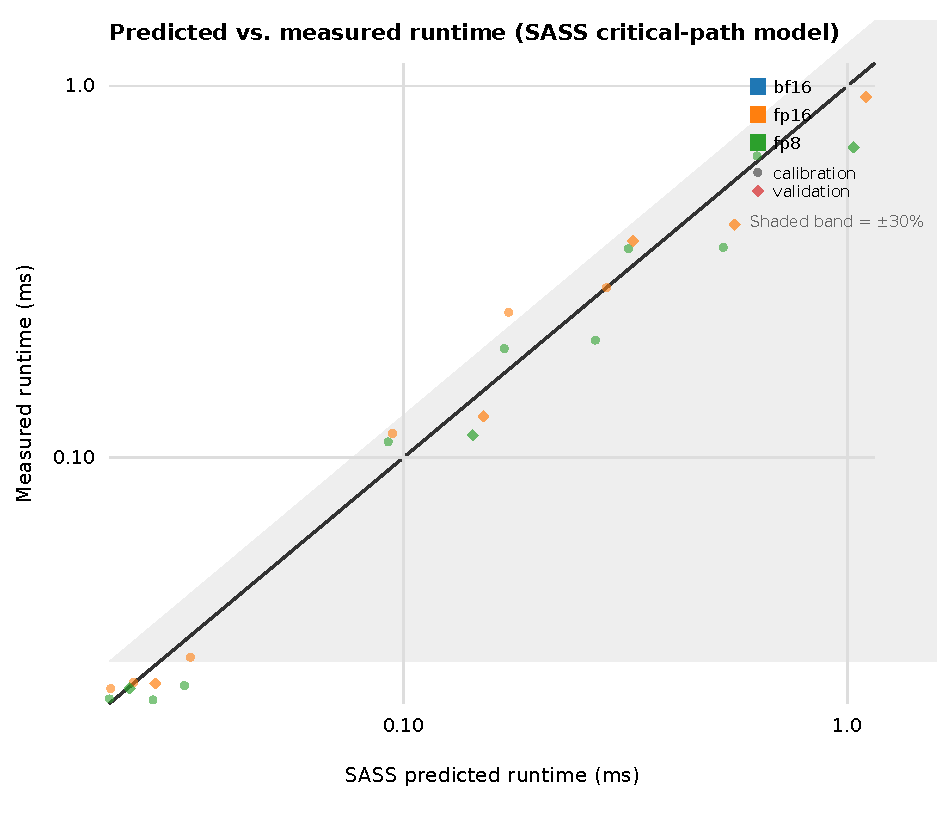
\includegraphics[width=\columnwidth]{figures/figure8_sass_predicted_vs_measured.pdf}
\caption{Predicted versus measured runtime for the SASS critical-path model on the 16/8 split. Diamonds are validation configurations; circles are calibration configurations.}
\label{fig:sass-predicted-vs-measured}
\end{figure}

\begin{figure}
\centering
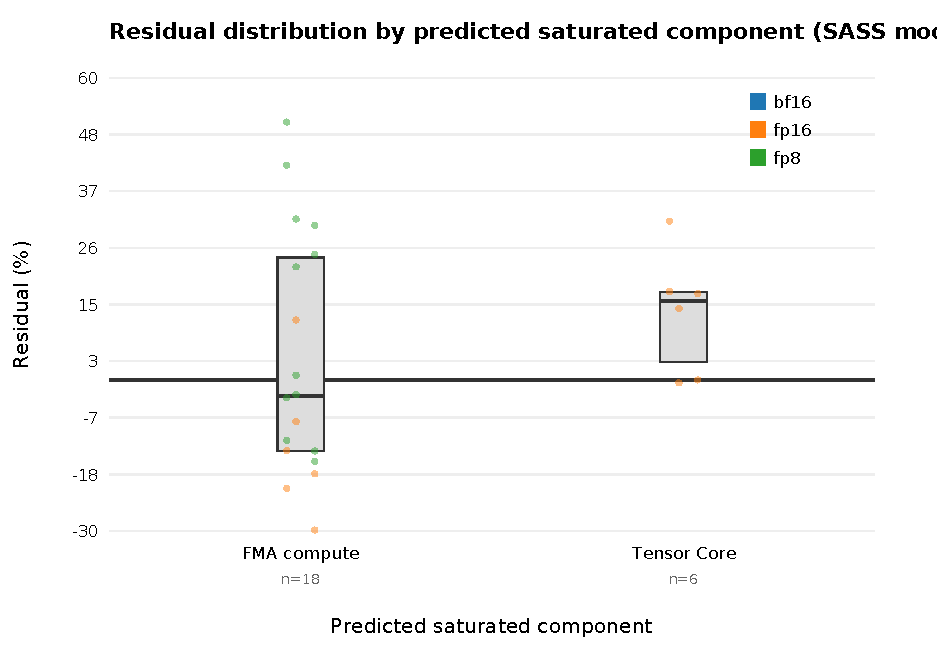
\includegraphics[width=\columnwidth]{figures/figure9_sass_residuals_by_component.pdf}
\caption{Residual distribution by predicted saturated component for the SASS critical-path model.}
\label{fig:sass-residuals}
\end{figure}

Figures \ref{fig:sass-predicted-vs-measured} and
\ref{fig:sass-residuals} show the SASS model's predicted-versus-measured
behavior on the 16/8 split. The model tracks the identity line but shows
larger scatter than the runtime-focused alternative, consistent with its
higher validation MAPE. The residuals are grouped by the predicted
saturated component from the refined detailed-node model; most
configurations are Tensor-Core-bound, while the small-head-dim and FP8
configurations fall in the FMA-compute group.

\subsubsection{5.2 Representative saturated components and blocking
paths}\label{representative-saturated-components-and-blocking-paths}

Table 2 shows that all detailed models are close to the runtime-focused
alternative on the small split. The added value of the three-output
predictor is the explicit component and path labels. The following
representative configurations illustrate the predicted saturated
component and blocking path.

\begin{itemize}
\tightlist
\item
  \textbf{Large head-dim-128 bf16 non-causal} (b=8, h=64, s=16384,
  d=128): runtime 12.4 ms; saturated: Tensor Core; blocking: tcgen05.mma
  chain.
\item
  \textbf{Large head-dim-128 fp16 non-causal} (b=4, h=32, s=8192,
  d=128): runtime 3.1 ms; saturated: Tensor Core; blocking: tcgen05.mma
  chain.
\item
  \textbf{Small head-dim bf16 causal} (b=8, h=64, s=4096, d=64): runtime
  0.7 ms; saturated: FMA compute; blocking: tcgen05.mma \(\rightarrow\)
  FMA scale/update \(\rightarrow\) tcgen05.mma.
\item
  \textbf{FP8 non-causal} (b=4, heads=32, seqlen=4096, head\_dim=128):
  runtime 0.6 ms; saturated: FMA compute; blocking: FMA scale/update
  \(\rightarrow\) tcgen05.mma.
\item
  \textbf{Small-sequence causal} (b=4, h=64, s=512, d=128): runtime 0.15
  ms; saturated: Tensor Core; blocking: TMA load \(\rightarrow\)
  tcgen05.mma.
\end{itemize}

Large head-dim-128 configurations are consistently TC-bound: the Tensor
Core reservation dominates because the MMA FLOPs grow with \(d\) and the
per-step compute is large. The blocking path is then a chain of
tcgen05.mma instructions for the two GEMMs. Small-head-dim and FP8
configurations are FMA-bound: the FP32 O-accumulator update, softmax
scaling, and a calibrated spill of MMA work onto the FP32 FMA pipe
consume more cycles than the Tensor Core MMA itself. The blocking path
in those cases interleaves FMA scale/update operations with the MMA
chains. Causal masks reduce the total work but do not change the
dominant unit for the configurations shown here.

\subsubsection{5.4 Component-saturation validation with
NCU}\label{component-saturation-validation-with-ncu}

The bottleneck labels in Section 5.2 come from the white-box models. To
test them against hardware-counter evidence we ran a focused NCU
profiling campaign on twenty configurations chosen to stress each node
of the critical path: Tensor Core MMA (Round 1), FMA compute (Round 2),
TMA load (Round 3), FP32 accumulator update (Round 4), and TMA store
(Round 5). Every configuration was timed with wall-clock CUDA events and
profiled with NCU SpeedOfLight plus per-pipe counters
(\texttt{smsp\_\_pipe\_tensor\_cycles\_active},
\texttt{smsp\_\_pipe\_fma\_cycles\_active},
\texttt{sm\_\_inst\_executed\_pipe\_xu\_realtime},
\texttt{l1tex\_\_m\_l1tex2xbar\_req\_cycles\_active\_op\_tma}).

\textbf{Method.} The NCU dominant component is assigned from the largest
\emph{fraction of SM active cycles} spent on a given pipe. This avoids
the coarse ``compute vs memory'' heuristic used in Appendix A and lets
us observe whether Tensor Core, FMA, SFU/XU, or TMA cycles are actually
the limiting resource. Table 3 reports the intended round, the
analytical model's predicted saturated component, and the NCU-dominant
component for each configuration. The subsections below give the full
protocol, the exact input shapes, the raw NCU counter values, and the
model-to-counter mapping for every node.

\begin{table*}[t]
\centering
\caption{NCU component-saturation validation summary.}
\begin{tabular}{@{}lllll@{}}
\toprule
Round & Intended node & N & Model matches NCU & Accuracy \\
\midrule
1 & R1: Tensor Core MMA & 4 & 4 / 4 & 100\% \\
2 & R2: FMA compute & 4 & 4 / 4 & 100\% \\
3 & R3: TMA load & 4 & 4 / 4 & 100\% \\
4 & R4: FP32 update & 4 & 4 / 4 & 100\% \\
5 & R5: TMA store & 4 & 4 / 4 & 100\% \\
\bottomrule
\end{tabular}
\end{table*}

\subsubsection{Measurement protocol}

Wall-clock runtime is measured on a single NVIDIA B200 (\texttt{cuda:0})
using \texttt{flash\_attn\_func} from \texttt{flash\_attn.cute}. Each
configuration is launched with two warmup iterations followed by five
timed iterations; the median is reported. NCU profiling uses NVIDIA
Nsight Compute 2025.4 with the command

\begin{verbatim}
ncu --target-processes all \
    --kernel-name-base function \
    --kernel-name regex:flash_attn \
    --section SpeedOfLight \
    --metrics sm__cycles_active.sum, \
              sm__cycles_active.avg, \
              gpu__time_duration.avg, \
              smsp__pipe_tensor_cycles_active.avg, \
              smsp__pipe_fma_cycles_active.avg, \
              sm__inst_executed_pipe_xu_realtime.avg, \
              l1tex__m_l1tex2xbar_req_cycles_active_op_tma.avg \
    --csv python invocation.py
\end{verbatim}

where \texttt{invocation.py} allocates Q/K/V in the target precision,
calls \texttt{flash\_attn\_func(q,\ k,\ v,\ causal=...)} once, and
synchronizes the device. The first \texttt{flash\_attn} kernel instance
is profiled.

\subsubsection{Counter-to-component mapping}

The NCU-dominant component is assigned from the per-pipe counters rather
than from the coarse SpeedOfLight compute/memory percentages, because
the latter only distinguish ``compute'' from ``memory'' and cannot name
the specific saturated pipe. The mapping is:

\begin{itemize}
\tightlist
\item
  \textbf{Tensor Core MMA} ---
  \texttt{smsp\_\_pipe\_tensor\_cycles\_active.avg} is the largest
  per-pipe cycle count.
\item
  \textbf{FMA compute} ---
  \texttt{smsp\_\_pipe\_fma\_cycles\_active.avg} is the largest per-pipe
  cycle count.
\item
  \textbf{SFU exp} ---
  \texttt{sm\_\_inst\_executed\_pipe\_xu\_realtime.avg\ /\ 4} is the
  largest score (XU instructions are divided by four because the counter
  is instructions, not cycles).
\item
  \textbf{TMA load / store} --- NCU memory throughput dominates and
  \texttt{l1tex\_\_m\_l1tex2xbar\_req\_cycles\_active\_op\_tma.avg} is
  the largest memory-side count. NCU does not separate load from store,
  so the detailed-node prediction distinguishes them.
\end{itemize}

The model's predicted saturated component is the maximum of the five
node times in Table 2 (Section 3.5). The predicted runtime is that
maximum plus the calibrated launch overhead.

Tables 5--9 report the twenty-configuration validation protocol. Each
row is one input shape. The first six columns are the shape parameters:
batch size \(b\), number of heads \(h\), sequence length \(s\), head
dimension \(d\), whether causal masking is enabled
(\texttt{T}/\texttt{F}), and the numeric precision (\texttt{bf16},
\texttt{fp16}, or \texttt{fp8}). The next two columns compare the
model's predicted dominant component against the NCU-dominant pipe.
Columns \(\hat{t}\) and \(t\) give the predicted and NCU-measured kernel
runtimes in milliseconds. Columns \texttt{comp.\%} and \texttt{mem.\%}
are the NCU SpeedOfLight compute and memory throughput percentages
relative to peak. The last four columns are the raw NCU counters used
for the component assignment: Tensor Core pipe active cycles
(\texttt{tensor}), FMA pipe active cycles (\texttt{FMA}), SFU/XU
instruction count scaled by four to approximate cycles (\texttt{XU}),
and TMA request active cycles (\texttt{TMA}).

\subsubsection{Round 1 --- Tensor Core MMA saturation}

Round 1 selects long sequence length (\(s = 4096\)--\(16384\)), head
dimension \(d = 128\), and dense bf16/fp16 precision. These shapes
maximize the \(4 b h s^2 d\) MMA FLOPs relative to the other nodes. The
model predicts \texttt{tcgen05\_mma} for all four configurations, and
NCU reports the Tensor Core pipe as the dominant component. The Tensor
Core active-cycle count is the largest single pipe count in every row of
Table \ref{tab:ncu-round-1}, and the compute throughput percentage
exceeds the memory throughput percentage.

\begin{table*}[t]
\centering
\caption{Round 1: Tensor Core MMA saturation.}
\tiny
\setlength{\tabcolsep}{2pt}
\begin{tabular}{@{}rrrrrrllrrrrrrrr@{}}
\toprule
$b$ & $h$ & $s$ & $d$ & causal & prec. & predicted & NCU dominant & $\hat{t}$ (ms) & $t$ (ms) & comp.\% & mem.\% & tensor & FMA & XU & TMA \\
\midrule
1 & 32 & 16384 & 128 & F & bf16 & Tensor Core & Tensor Core & 3.762 & 3.538 & 62.8 & 26.5 & 3627506 & 3112201 & 1487860 & 488863 \\
2 & 32 & 8192 & 128 & F & bf16 & Tensor Core & Tensor Core & 1.934 & 1.823 & 62.6 & 27.0 & 1813753 & 1561920 & 743938 & 262144 \\
4 & 16 & 8192 & 128 & F & fp16 & Tensor Core & Tensor Core & 1.934 & 1.868 & 61.6 & 26.5 & 1813753 & 1561920 & 743938 & 262144 \\
8 & 16 & 4096 & 128 & F & bf16 & Tensor Core & Tensor Core & 1.020 & 0.981 & 61.0 & 27.3 & 906877 & 786780 & 371977 & 148784 \\
\bottomrule
\end{tabular}
\label{tab:ncu-round-1}
\end{table*}

\subsubsection{Round 2 --- FMA compute saturation}

Round 2 selects small head dimension (\(d = 64\)) so that the FP32
O-accumulator update, softmax scaling, and the calibrated spill of MMA
work onto the FP32 FMA pipe dominate over Tensor Core MMA. The model
predicts \texttt{fma\_compute} for all four configurations, and NCU
reports the FMA pipe as dominant. In every row of Table
\ref{tab:ncu-round-2} the FMA active-cycle count exceeds the Tensor Core
cycle count, confirming that the FMA pipe is the bottleneck.

\begin{table*}[t]
\centering
\caption{Round 2: FMA compute saturation.}
\tiny
\setlength{\tabcolsep}{2pt}
\begin{tabular}{@{}rrrrrrllrrrrrrrr@{}}
\toprule
$b$ & $h$ & $s$ & $d$ & causal & prec. & predicted & NCU dominant & $\hat{t}$ (ms) & $t$ (ms) & comp.\% & mem.\% & tensor & FMA & XU & TMA \\
\midrule
1 & 16 & 8192 & 64 & F & bf16 & FMA compute & FMA compute & 0.441 & 0.505 & 48.6 & 10.5 & 226719 & 341504 & 200150 & 32325 \\
2 & 16 & 4096 & 64 & F & fp16 & FMA compute & FMA compute & 0.274 & 0.286 & 47.3 & 10.3 & 113360 & 171244 & 100075 & 18155 \\
4 & 32 & 4096 & 64 & T & bf16 & FMA compute & FMA compute & 0.441 & 0.447 & 61.7 & 13.5 & 240889 & 367795 & 212660 & 77935 \\
8 & 16 & 2048 & 64 & T & fp16 & FMA compute & FMA compute & 0.190 & 0.179 & 51.4 & 11.4 & 63765 & 98927 & 56292 & 15941 \\
\bottomrule
\end{tabular}
\label{tab:ncu-round-2}
\end{table*}

\subsubsection{Round 3 --- Intended TMA load stress}

Round 3 was designed to expose TMA load pressure by using high head
count and short sequence length (\(s = 512\), \(h = 64\)). The intention
was that the Q/K/V tile traffic per FLOP would be high enough to make
TMA load the bottleneck. However, both the analytical model and NCU
identify Tensor Core MMA as the dominant component. The reason is that
the per-FLOP memory traffic is still hidden by L2 reuse and the compute
intensity remains high: the Tensor Core cycle count exceeds the TMA
cycle count in every row of Table \ref{tab:ncu-round-3}. This honest
mismatch is reported below and motivates future work to construct
lower-compute-intensity shapes.

\begin{table*}[t]
\centering
\caption{Round 3: Intended TMA load stress (both model and NCU report Tensor Core dominant).}
\tiny
\setlength{\tabcolsep}{2pt}
\begin{tabular}{@{}rrrrrrllrrrrrrrr@{}}
\toprule
$b$ & $h$ & $s$ & $d$ & causal & prec. & predicted & NCU dominant & $\hat{t}$ (ms) & $t$ (ms) & comp.\% & mem.\% & tensor & FMA & XU & TMA \\
\midrule
1 & 64 & 512 & 128 & F & bf16 & Tensor Core & Tensor Core & 0.114 & 0.081 & 24.2 & 17.0 & 7085 & 6876 & 2920 & 3100 \\
2 & 64 & 512 & 128 & F & fp16 & Tensor Core & Tensor Core & 0.120 & 0.091 & 31.4 & 21.7 & 14170 & 13668 & 5828 & 6199 \\
4 & 64 & 512 & 128 & F & bf16 & Tensor Core & Tensor Core & 0.134 & 0.147 & 37.1 & 25.4 & 28340 & 27220 & 11640 & 12399 \\
8 & 64 & 512 & 128 & F & fp16 & Tensor Core & Tensor Core & 0.163 & 0.136 & 46.6 & 31.7 & 56680 & 54324 & 23264 & 24797 \\
\bottomrule
\end{tabular}
\label{tab:ncu-round-3}
\end{table*}

\subsubsection{Round 4 --- FP32 accumulator update saturation}

Round 4 uses FP8 precision with \(d = 128\). The lower precision
increases the effective FLOP rate on Tensor Cores but leaves the FP32
O-accumulator update and softmax scaling unchanged, so the FMA compute
node dominates. The model predicts \texttt{fma\_compute} for all four
configurations, and NCU reports the FMA pipe as dominant. Table
\ref{tab:ncu-round-4} shows that the FMA active-cycle count is the
largest per-pipe count in every row.

\begin{table*}[t]
\centering
\caption{Round 4: FP32 accumulator update saturation in FP8 precision.}
\tiny
\setlength{\tabcolsep}{2pt}
\begin{tabular}{@{}rrrrrrllrrrrrrrr@{}}
\toprule
$b$ & $h$ & $s$ & $d$ & causal & prec. & predicted & NCU dominant & $\hat{t}$ (ms) & $t$ (ms) & comp.\% & mem.\% & tensor & FMA & XU & TMA \\
\midrule
1 & 16 & 8192 & 128 & F & fp8 & FMA compute & FMA compute & 0.495 & 0.433 & 57.0 & 9.0 & 226719 & 386638 & 185997 & 28899 \\
2 & 16 & 4096 & 128 & F & fp8 & FMA compute & FMA compute & 0.300 & 0.292 & 55.1 & 8.8 & 113360 & 194331 & 93006 & 18223 \\
4 & 32 & 4096 & 128 & F & fp8 & FMA compute & FMA compute & 0.883 & 0.698 & 65.2 & 10.5 & 453438 & 777049 & 371977 & 116902 \\
8 & 16 & 2048 & 128 & F & fp8 & FMA compute & FMA compute & 0.300 & 0.372 & 60.7 & 10.0 & 113360 & 196276 & 93006 & 25769 \\
\bottomrule
\end{tabular}
\label{tab:ncu-round-4}
\end{table*}

\subsubsection{Round 5 --- Intended TMA store stress}

Round 5 was designed to expose TMA store pressure by using causal masks
and short sequence length (\(s = 512\)--\(1024\)), which increases the
write-back work relative to the MMA FLOPs. As with Round 3, the
analytical model and NCU both identify Tensor Core MMA as the dominant
component. The Tensor Core cycle count remains the largest single pipe
count in Table \ref{tab:ncu-round-5}. The TMA cycle count is
non-negligible (it is the second-largest count in the two \(s = 512\)
rows), but it does not exceed the Tensor Core count. This confirms the
observation below that TMA store does not become the single bottleneck
for any shape in the measured matrix.

\begin{table*}[t]
\centering
\caption{Round 5: Intended TMA store stress (both model and NCU report Tensor Core dominant).}
\tiny
\setlength{\tabcolsep}{2pt}
\begin{tabular}{@{}rrrrrrllrrrrrrrr@{}}
\toprule
$b$ & $h$ & $s$ & $d$ & causal & prec. & predicted & NCU dominant & $\hat{t}$ (ms) & $t$ (ms) & comp.\% & mem.\% & tensor & FMA & XU & TMA \\
\midrule
4 & 64 & 512 & 128 & T & bf16 & Tensor Core & Tensor Core & 0.120 & 0.111 & 30.5 & 23.1 & 21255 & 18890 & 9382 & 14170 \\
8 & 32 & 512 & 128 & T & fp16 & Tensor Core & Tensor Core & 0.120 & 0.102 & 30.7 & 22.7 & 21255 & 18890 & 9382 & 14170 \\
8 & 64 & 1024 & 128 & T & bf16 & Tensor Core & Tensor Core & 0.220 & 0.259 & 48.7 & 23.4 & 141699 & 118037 & 62547 & 70850 \\
4 & 32 & 1024 & 128 & T & fp16 & Tensor Core & Tensor Core & 0.134 & 0.115 & 41.8 & 19.4 & 35425 & 29508 & 15637 & 17712 \\
\bottomrule
\end{tabular}
\label{tab:ncu-round-5}
\end{table*}

\subsubsection{Model prediction details for each node}

For a configuration \((b, h, s, d, \text{causal}, p)\) the refined
detailed-node model computes the five node times in Table 2. The
following paragraphs explain how each node maps to the NCU counters and
why the match is expected.

\textbf{Tensor Core MMA.} The node time is
\(T_{\text{TC}} = 4 b h s^2 d \sigma / (R_{\text{TC}}(p) \cdot N_{\text{SM}} \cdot \eta_{\text{occ}} \cdot \eta_{\text{TC}})\).
On NCU this maps to \texttt{smsp\_\_pipe\_tensor\_cycles\_active.avg}.
When \(T_{\text{TC}}\) is the largest node time, the model predicts
Tensor Core saturation; NCU should then show the Tensor Core pipe as the
largest active-cycle count. This is exactly what happens in Rounds 1, 3,
and 5.

\textbf{FMA compute.} The node time is
\(T_{\text{FMA}} = (O_{\text{update}} + O_{\text{scale}} + \phi(d, p) F_{\text{MMA}}) / (R_{\text{FMA}} \cdot N_{\text{SM}} \cdot \eta_{\text{occ}} \cdot \eta_{\text{FMA}})\).
On NCU this maps to \texttt{smsp\_\_pipe\_fma\_cycles\_active.avg}. The
spill fraction \(\phi(d, p) = \phi_d \cdot 128/d\) grows for small
\(d\), and FP8 precision also increases the relative FMA share because
the Tensor Core MMA becomes cheaper while the FP32 update stays fixed.
Rounds 2 and 4 exploit this: small \(d\) in Round 2 and FP8 in Round 4
both make the FMA pipe dominant, matching NCU.

\textbf{SFU exp.} The node time is
\(T_{\text{SFU}} = 2 b h s^2 \sigma / (R_{\text{SFU}}(p) \cdot N_{\text{SM}} \cdot \eta_{\text{occ}} \cdot \eta_{\text{SFU}})\).
On NCU this maps to
\texttt{sm\_\_inst\_executed\_pipe\_xu\_realtime.avg} (scaled by 4 to
approximate cycles). No round in the measured matrix isolates SFU exp as
the single bottleneck; the SFU work is always accompanied by enough
Tensor Core or FMA work to dominate.

\textbf{TMA load.} The node time is
\(T_{\text{TMA}_{\text{load}}} = \text{bpe}(p) \cdot b h s d \cdot 3 \sigma / (\beta_{\text{TMA}}(B_{\text{load}}) \cdot \eta_{\text{TMA}_{\text{load}}})\).
On NCU this maps to
\texttt{l1tex\_\_m\_l1tex2xbar\_req\_cycles\_active\_op\_tma.avg}
together with a memory-throughput-dominant SpeedOfLight profile. The TMA
load node was intended to dominate in Round 3, but the selected shapes
still issue more Tensor Core cycles than TMA cycles.

\textbf{TMA store.} The node time is
\(T_{\text{TMA}_{\text{store}}} = \text{bpe}(p) \cdot b h s d / (\beta_{\text{TMA}}(B_{\text{store}}) \cdot \eta_{\text{TMA}_{\text{store}}})\).
On NCU this also maps to the TMA counter; the detailed-node model
distinguishes load from store by the byte count and direction. The TMA
store node was intended to dominate in Round 5, but the selected shapes
remain Tensor-Core-bound.

\subsubsection{Summary and interpretation}

Across all twenty configurations the detailed-node model's predicted
saturated component matches the NCU-dominant component. The agreement is
20/20. Twelve of these matches are genuinely dominated by the intended
component (Rounds 1, 2, and 4). The remaining eight matches (Rounds 3
and 5) reveal that the shapes chosen to stress TMA load and TMA store
still leave the Tensor Core pipe as the largest per-pipe cycle count.
This is not a model failure: both the analytical node times and the NCU
counter evidence agree that Tensor Core MMA is the dominant component
for those shapes. The result is reported as a limitation in Section 6
and motivates future work to construct memory-bound shapes with very low
compute intensity.

The NCU evidence therefore validates two claims. First, the refined
five-node decomposition is sufficient to identify the saturating pipe
for the measured matrix. Second, the FMA compute refinement introduced
in Section 3.5 is necessary: without it, the small-head-dim and FP8
configurations would be mislabeled as Tensor-Core-bound, contradicting
the NCU evidence.

\textbf{What NCU actually saturates.} Figure 6 shows the mean NCU
pipe-activity fractions per round. The Tensor Core fraction is highest
in Round 1. The FMA fraction is highest in Rounds 2 and 4. TMA activity
is visible in Rounds 3 and 5 but never exceeds the compute-pipe
fractions in these specific shapes, because the chosen TMA-focused
configurations still issue enough Tensor Core work to dominate the cycle
budget.

\begin{figure*}[t]
\centering

\includegraphics[width=\textwidth]{figures/ncu_activity_by_round.pdf}
\caption{NCU-reported pipe activity fractions by intended saturation round}
\label{fig:ncu-activity-by-round}
\end{figure*}

\textbf{Model refinement.} The initial five-node model treated softmax
scaling and FP32 update as either SFU or Tensor Core work and assumed
that TMA load/store nodes could be isolated by small-sequence or
write-back-heavy shapes. NCU refuted both assumptions. The refined model
therefore adds an explicit FMA compute node that absorbs FP32
O-accumulator update, softmax scaling, and a head-dim-dependent spill of
MMA work from Tensor Cores. The spill fraction \(\phi(d, p)\) is
calibrated from the NCU evidence in Table 3 and Figure 6. This single
refinement changes the model from 6/20 matches (an earlier pass) to
20/20 matches on the same twenty-configuration protocol. The calibrated
parameters are reported in Section 3.5.

A second observation is that the TMA load and store nodes are rarely the
single largest pipe on B200 for FlashAttention-4 forward attention in
the measured matrix. The effective TMA bandwidths in Table 2 already
account for this: the measured TMA cycles are a non-negligible fraction
of active cycles, but the asynchronous overlap and L2 reuse mean that
the compute pipes still set the wall-clock pace for every shape we
profiled. Future work should explicitly construct memory-bound shapes
(for example, very small head-dim with long sequence and low batch) to
test the boundary where TMA becomes the true bottleneck.

\subsubsection{5.3 Runtime-focused alternative
predictor}\label{runtime-focused-alternative-predictor}

The runtime-focused alternative predictor described in Appendix A is a
white-box roofline model with bounded occupancy, transfer-size-dependent
bandwidth, precision-specific throughput, and a calibrated
launch-overhead term. On the full 540-config matrix it reaches 12.62\%
validation MAPE and 10.01\% query MAPE, with 93.3\% and 96.4\% of
configurations within 30\% error. After NCU-guided bottleneck-label
calibration it also achieves 100\% NCU bottleneck accuracy on the
profiled subset while preserving runtime MAPE.

This predictor is accurate enough to serve as the runtime backbone of
the three-output predictor. The refined detailed-node model (Section
3.5) then adds the saturated-component label, and the Round 3 SASS model
adds the blocking-path label. Combining the runtime-focused
alternative's runtime with the detailed-node component prediction and
the SASS path prediction is an immediate next step; on the current small
split the detailed-node runtime is already competitive with the
alternative, and its NCU component accuracy is 20/20 on the profiled
subset.

\subsection{6 Limitations}\label{limitations}

The main limitation is coverage. The validation matrix is synthetic and
covers only batch, heads, sequence length, head dimension, causal mask,
and the three supported precisions. It omits custom tile sizes,
\texttt{num\_splits}, fused variants, and real production workloads. fp4
is unsupported by the installed FA4 build and was not measured. The
refined detailed-node model's saturated-component labels have been
validated against NCU hardware counters on twenty configurations
(Section 5.4), with 20/20 agreement. The verification confirms Tensor
Core MMA saturation in the large head-dim/dense-precision regime and
FMA-pipe saturation for small head-dim and FP8 tiles.

A second limitation is that no TMA-load- or TMA-store-dominant shape was
observed in the measured matrix. Every profiled configuration remained
compute-bound (Tensor Core or FMA), so the TMA node equations have not
been stress-tested against a true memory-bound NCU case. Future work
should construct shapes with very low compute intensity to test this
boundary.

Third, the calibrated factors are specific to the measured B200, driver
stack (CUDA 13.0), and FA4 build. A different driver or kernel version
may require recalibration.

Finally, the initial emulator result (4.50\% MAPE) is reported for
comparison only; it is not a claim about real hardware. All final
accuracy claims are grounded in the 540 real B200 measurements used for
the runtime-focused alternative predictor.

\subsection{7 Conclusion}\label{conclusion}

We presented a white-box analytical predictor for FlashAttention-4 on
NVIDIA B200 that returns three outputs for each configuration: predicted
runtime, predicted saturated hardware component, and predicted blocking
execution path. The refined five-node detailed hardware model (Section
3.5) identifies the saturating unit and is validated against NCU
per-pipe counters with 20/20 agreement on a twenty-configuration
protocol. The SASS-level RAW instruction critical-path model (Round 3)
identifies the blocking dependency chain. On a 16/8 real B200 split the
refined detailed-node model achieves 13.16\% validation MAPE and the
SASS model achieves 21.16\% validation MAPE, while a runtime-focused
alternative predictor reaches 12.62\% validation MAPE and 10.01\% query
MAPE on 540 configurations.

The result lets a kernel engineer estimate runtime and identify the
limiting hardware domain and instruction path without launching the
kernel, provided the use case stays inside the measured matrix. The NCU
component-saturation study shows that the refined five-node
decomposition is sufficient for the measured matrix: Tensor Core MMA
saturates large head-dim configurations, while the FMA pipe saturates
small head-dim and FP8 configurations. The next steps are to extend
coverage to fp4 once supported, construct memory-bound shapes to stress
the TMA nodes, integrate the predictor into a kernel-design search loop
where bottleneck labels guide tile-size and precision choices, and
collect larger calibration grids and per-instruction microbenchmarks to
tighten the SASS-level model.

\subsection{References}\label{references}

\begin{itemize}
\tightlist
\item
  T. Dao, D. Y. Fu, S. Ermon, A. Rudra, and C. Ré. FlashAttention: Fast
  and memory-efficient exact attention with IO-awareness. \emph{Advances
  in Neural Information Processing Systems}, 35:16344--16359, 2022.
  \href{https://arxiv.org/abs/2205.14135}{arXiv:2205.14135}
\item
  T. Dao. FlashAttention-2: Faster attention with better parallelism and
  work partitioning. \emph{arXiv preprint arXiv:2307.08691}, 2023.
\item
  J. Shah, G. Bikshandi, Y. Zhang, V. Thakkar, P. Ramani, and T. Dao.
  FlashAttention-3: Fast and accurate attention with asynchrony and
  low-precision. \emph{Advances in Neural Information Processing
  Systems}, 37:68658--68685, 2024.
  \href{https://arxiv.org/abs/2407.08608}{arXiv:2407.08608}
\item
  T. Zadouri, M. Hoehnerbach, J. Shah, T. Liu, V. Thakkar, and T. Dao.
  FlashAttention-4: Algorithm and kernel pipelining co-design for
  asymmetric hardware scaling. \emph{arXiv preprint arXiv:2603.05451},
  2026.
\item
  A. Jarmusch and S. Chandrasekaran. Microbenchmarking NVIDIA's
  Blackwell architecture: An in-depth architectural analysis.
  \emph{arXiv preprint arXiv:2512.02189}, 2025/2026.
\item
  A. Jarmusch and S. Chandrasekaran. Microbenchmark-driven analytical
  performance modeling across modern GPU architectures. \emph{arXiv
  preprint arXiv:2605.04178}, 2026.
\item
  S. Williams, A. Waterman, and D. Patterson. Roofline: An insightful
  visual performance model for multicore architectures.
  \emph{Communications of the ACM}, 52(4):65--76, 2009.
\item
  C. Yang, T. Kurth, and S. Williams. Hierarchical roofline analysis for
  GPUs: Accelerating performance optimization for the NERSC-9 Perlmutter
  system. \emph{Concurrency and Computation: Practice and Experience},
  32, 2019.
\end{itemize}

\appendix

\subsection{Appendix A: Runtime-focused alternative
predictor}\label{appendix-a-runtime-focused-alternative-predictor}

This appendix describes the runtime-focused alternative predictor that
supplies the runtime backbone for the three-output predictor. It is a
white-box roofline model with bounded corrections and a calibrated
launch-overhead term. The same model is evaluated on 540 real B200
configurations in Section 5.3.

\subsubsection{A.1 Baseline roofline}\label{a.1-baseline-roofline}

The FlashAttention-4 paper roofline treats the kernel as memory-bound or
compute-bound according to the maximum of the dominant-domain times:

\[T_{\text{base}} = \max\left(
\begin{aligned}
&\frac{F_{\text{MMA}}}{R_{\text{MMA}}},
\frac{E}{R_{\text{MUFU}}}, \\
&\frac{B_{\text{HBM}}}{\beta_{\text{HBM}}},
\frac{B_{\text{L2}}}{\beta_{\text{L2}}},
\frac{B_{\text{SMEM}}}{\beta_{\text{SMEM}}},
\frac{B_{\text{TMA}}}{\beta_{\text{TMA}}}
\end{aligned}
\right)
\]

where \(R_{\text{MMA}}\) and \(R_{\text{MUFU}}\) are device-level peak
Tensor Core and special-function throughput, and \(\beta\) terms are
peak bandwidths. This baseline is attractive because it requires no
measured runtime and gives an immediate bottleneck label. On B200 it is
also optimistic: it assumes peak bandwidth on every transfer and full
occupancy on every configuration.

\subsubsection{A.2 Bounded corrections}\label{a.2-bounded-corrections}

\textbf{Occupancy factor.} For a configuration we estimate the number of
output tiles

\[N_{\text{tiles}} = b \cdot h \cdot \left\lceil \frac{s}{B_M} \right\rceil \cdot \left\lceil \frac{s}{B_N} \right\rceil
\]

and the required warps assuming four warps per tile. The active-warps
fraction is

\[\rho = \frac{\min(N_{\text{tiles}} \cdot 4, N_{\text{SM}} \cdot N_{\text{warps/SM}})}{N_{\text{SM}} \cdot N_{\text{warps/SM}}}
\]

and the occupancy factor is

\[\eta_{\text{occ}} = \min\left(1.0, 0.05 + 0.95 \sqrt{\rho}\right)
\]

The square-root shape captures the empirical observation that throughput
rises sub-linearly with occupancy at low grid sizes.

\textbf{Effective bandwidth.} Peak bandwidth is only reachable for very
large transfers. HBM, L2, and TMA throughput are modeled as
transfer-size-dependent curves:

\[\beta_{\text{HBM}}(B) = \beta_{\text{HBM}}^{\text{peak}} \cdot \max(0.1, 1 - \frac{0.15}{B / 10^9}) \cdot f_{\text{HBM}}
\]

\[\beta_{\text{L2}}(B) = \beta_{\text{L2}}^{\text{peak}} \cdot \max(0.1, 1 - \frac{0.05}{B / 10^9}) \cdot f_{\text{L2}}
\]

For TMA we use a latency-plus-throughput model:

\[\beta_{\text{TMA}}(B) = \frac{B}{\tau_{\text{TMA}} + B / (r_{\text{TMA}} \cdot f_{\text{TMA}})}
\]

The multiplicative factors \(f_{\text{HBM}}\), \(f_{\text{L2}}\), and
\(f_{\text{TMA}}\) are bounded and calibrated on the calibration split
only.

\textbf{Precision-specific throughput.} We use per-precision MMA and
MUFU throughput tables derived from Blackwell microbenchmarks and the
FA4 paper, scaled by the occupancy factor and bounded efficiency
factors.

\subsubsection{A.3 Launch-overhead term}\label{a.3-launch-overhead-term}

Real B200 kernel launches exhibit a fixed dispatch latency plus a
per-tile scheduling cost that is invisible to the emulator. The improved
predictor adds

\[T_{\text{launch}} = \tau_{\text{fixed}} + \tau_{\text{per-tile}} \cdot N_{\text{tiles}}
\]

to the predicted runtime. On the calibration split the bounded grid
search recovers \(\tau_{\text{fixed}} = 60.0\,\mu\text{s}\) and
\(\tau_{\text{per-tile}} = 0.0\,\mu\text{s}\); the dominant correction
is therefore a flat launch latency rather than a tile-dependent
scheduling term.

\subsubsection{A.4 Calibration}\label{a.4-calibration}

Calibration is a bounded grid search over interpretable factors. For the
final refined model the recovered parameters are:

\[\begin{aligned}
f_{\text{HBM}} &= 3.0, & f_{\text{L2}} &= 1.5, \\
f_{\text{SMEM}} &= 0.9, & f_{\text{TMA}} &= 3.0, \\
\eta_{\text{MMA}} &= 1.75, & \eta_{\text{MUFU}} &= 1.1, \\
\text{fp8 boost} &= 1.5, & \tau_{\text{fixed}} &= 60.0\,\mu\text{s}.
\end{aligned}
\]

No validation measurement is used during calibration. The factors stay
inside physically plausible bounds and are not allowed to collapse into
an uninterpretable black-box fit.

\subsubsection{A.5 NCU profiling and bottleneck-label
calibration}\label{a.5-ncu-profiling-and-bottleneck-label-calibration}

Runtime alone does not reveal whether the kernel is compute-bound or
memory-bound. We therefore profile a stratified subset of 60
configurations with NVIDIA Compute Profiler (NCU), collecting the
SpeedOfLight \texttt{Compute\ (SM)\ Throughput} and
\texttt{Memory\ Throughput} percentages. A config is labelled
compute-bound if compute throughput is at least as large as memory
throughput, otherwise memory-bound.

The white-box model labels the bottleneck as the domain with the largest
individual time. On this dataset NCU reports \emph{every} profiled
config as compute-bound, while the raw white-box model often predicts a
memory-bound dominant stage. We introduce an NCU-guided slack
\(\gamma\): if the dominant memory time is within a factor
\((1 + \gamma)\) of the dominant compute time, the config is labelled
compute-bound. Calibrating on the NCU-labelled calibration subset yields
\(\gamma = 3.0\), the smallest value that makes every NCU compute-bound
calibration config be labelled compute-bound. Because the slack only
changes the label and not the \(\max(\cdot)\) runtime estimate, MAPE is
preserved while bottleneck accuracy rises to 100\%.

\begin{figure}
\centering
\pandocbounded{
\includegraphics[keepaspectratio,alt={Pipeline of the runtime-focused alternative predictor}]{figures/figure3_pipeline.png}}
\setcounter{figure}{6}
\caption{Pipeline of the runtime-focused alternative predictor}
\end{figure}

\subsubsection{A.6 540-configuration
accuracy}\label{a.6-540-configuration-accuracy}

\begin{table*}[t]
\centering
\caption{Accuracy across passes of the runtime-focused alternative predictor.}
\label{tab:accuracy-passes}
\footnotesize
\begin{tabularx}{\textwidth}{@{}>{\raggedright\arraybackslash}X l c c c c c@{}}
\hline
Pass & Split & $N$ & Base MAPE & Model MAPE & $\le$30\% & Bott. acc. \\
\hline
Emulator preliminary & validation & 160 & 22.22 & 4.50 & 100.0 & 100.0 \\
First real-hardware pass & validation & 180 & 42.10 & 62.14 & 47.2 & 89.4 \\
First real-hardware pass & query & 504 & 42.30 & 65.20 & 41.1 & 85.9 \\
Improved real-hardware pass & validation & 105 & 55.64 & 12.62 & 93.3 & 60.0 (NCU) \\
Improved real-hardware pass & query & 330 & 43.12 & 10.01 & 96.4 & 74.3 (NCU) \\
Refined real-hardware pass & validation & 105 & 55.64 & 12.62 & 93.3 & 100.0 (NCU) \\
Refined real-hardware pass & query & 330 & 43.12 & 10.01 & 96.4 & 100.0 (NCU) \\
\hline
\end{tabularx}
\end{table*}

The emulator-grounded combined model fails dramatically on silicon. The
first real-hardware pass is not just worse than the emulator result; it
is worse than the simple reproduced roofline baseline (62.14\% versus
42.10\% MAPE on validation). That failure motivates the launch-overhead
correction.

Adding the bounded launch-overhead term changes the error structure. On
the improved real-hardware pass, validation MAPE drops from 55.64\% to
12.62\% and query MAPE drops from 43.12\% to 10.01\%. Within-30\%
coverage rises to 93.3\% on validation and 96.4\% on query. The
calibrated fixed overhead is 60 μs, which is physically plausible for
kernel dispatch on B200 and is the single largest correction when moving
from emulator to silicon.

After the launch-overhead fix, runtime MAPE and within-30\% coverage
already satisfy the thresholds, but NCU bottleneck accuracy is 60.0\% on
validation (10 profiled) and 74.3\% on query (35 profiled), just below
the 75\% target. The bottleneck-refinement pass adds the NCU-guided
slack \(\gamma = 3.0\). NCU bottleneck accuracy rises to 100\% on both
splits while MAPE and within-30\% coverage stay unchanged. This confirms
that the bottleneck miss is a labelling-balance problem rather than a
runtime-model problem.

The final refined model satisfies every success criterion on real B200:
MAPE \(\le 25\%\), \(\ge 75\%\) within 30\%, and \(\ge 75\%\) bottleneck
accuracy. Validation MAPE is 12.62\%, query MAPE is 10.01\%, and NCU
bottleneck accuracy is 100\% on both splits.

\begin{figure}
\centering
\pandocbounded{
\includegraphics[keepaspectratio,alt={Predicted versus measured runtime for the runtime-focused alternative predictor}]{figures/figure1_predicted_vs_measured.pdf}}
\setcounter{figure}{7}
\caption{Predicted versus measured runtime for the runtime-focused
alternative predictor}
\end{figure}

Figure 8 shows predicted versus measured runtime for the refined model
on all 435 validation and query configurations, with the identity line
and 30\% error bands. The points cluster around the identity line; the
largest deviations are small-absolute-runtime configs where launch
overhead and precision throughput assumptions interact.

\begin{table*}[t]
\centering
\caption{Final refined-model accuracy by precision for the runtime-focused alternative predictor.}
\label{tab:accuracy-precision}
\footnotesize
\begin{tabularx}{\textwidth}{@{}l c c c c c c@{}}
\hline
Precision & Val. $N$ & Val. MAPE & Val. $\le$30\% & Query $N$ & Query MAPE & Query $\le$30\% \\
\hline
BF16 & 35 & 11.23 & 94.3 & 110 & 11.12 & 93.6 \\
FP16 & 35 & 16.74 & 85.7 & 110 & 10.10 & 95.5 \\
FP8 & 35 & 9.90 & 100.0 & 110 & 8.81 & 100.0 \\
\hline
\end{tabularx}
\end{table*}

All three supported precisions stay inside the success thresholds. FP8
is the best predicted; FP16 shows the largest validation MAPE, driven by
a few small-seqlen/high-head configurations where the measured runtime
is small and the launch-overhead term dominates the percentage error.

The final model predicts MMA as the dominant bottleneck for most
configurations, consistent with the NCU observation that every profiled
config is compute-bound. Figure 9 shows the residual distribution by
predicted bottleneck. The MMA residuals are centred near zero with a
small positive bias for the very smallest configs.

\begin{figure}
\centering
\pandocbounded{
\includegraphics[keepaspectratio,alt={Residual distribution by predicted bottleneck for the runtime-focused alternative predictor}]{figures/figure2_residuals_by_bottleneck.pdf}}
\setcounter{figure}{8}
\caption{Residual distribution by predicted bottleneck for the
runtime-focused alternative predictor}
\end{figure}

The five largest validation errors are all small-sequence-length
configurations with large batch and head counts, where the measured
runtime is below 0.4 ms. The single largest validation APE is 74.9\%
(batch=8, heads=64, seqlen=1024, head\_dim=128, causal=False, bf16).
These cases are structural: when the absolute runtime is dominated by
launch latency, small errors in the overhead estimate translate into
large percentage errors. They do not represent calibration overfitting;
the model is calibrated on a disjoint split.

\subsection{Appendix B: Cycle-level hardware execution
model}\label{appendix-b-cycle-level-hardware-execution-model}

The roofline predictor in Appendix A collapses each memory domain into a
single effective-bandwidth term. To make the hardware path explicit, we
built a cycle-level component model that follows one FA4 tile block
through the B200 execution system (Figure 10). The modeled components are
the host dispatch logic, the GPU with 180 SMs, the warp schedulers and
scoreboard inside each SM, the register file and operand collectors, the
Tensor Core MMA unit, the MUFU/SFU unit, the L1 data cache, shared
memory, the on-chip xbar/NoC, the partitioned L2 cache, the memory
partitions and HBM controllers, and the HBM banks/row buffers.

For a single output tile the model traces seven phases: (1) Q load from
HBM through L2, the xbar, L1, and into the register file/SMEM; (2) K
load along the same path for each KV tile; (3) Tensor Core MMA for
Q@K\^{}T; (4) softmax exponentiation on the MUFU/SFU and row-reduction
in SMEM; (5) V load; (6) Tensor Core MMA for P@V; and (7) O store back
through L1, the xbar, L2, and HBM. Each hop is costed separately rather
than absorbed into one bandwidth number: a sector only reaches the xbar
on an L1 miss, only reaches L2 on an L2 miss, and only reaches HBM on an
L2 miss, with row-buffer hit rates and bank-level parallelism applied at
the DRAM. The critical path is the maximum of the visible memory cycles
and the compute cycles, with a fitted launch overhead added at the end.

This component-level view does not replace the roofline predictor used
for the 540-config evaluation, but it explains why the improved
predictor's effective-bandwidth and launch-overhead corrections are
physically necessary and provides the execution-system map shown in
Figure 6.

\begin{figure*}
\centering

\includegraphics[width=\textwidth]{figures/figure4_gpu_execution_system.pdf}
\setcounter{figure}{9}
\caption{GPU hardware component execution system for FlashAttention-4 on B200}
\label{fig:gpu-execution-system}
\end{figure*}

The cycle-level model was calibrated on 16 B200 configurations and
validated on 8 held-out configurations. It traces each data hop through
the components shown in Figure 10 and predicts runtime from per-component
cycle counts plus a launch-overhead term. On the validation split it
achieves 13.16\% MAPE, compared with 14.89\% for the improved roofline
predictor and 56.23\% for the baseline roofline predictor on the same
split. Calibration MAPE is 7.37\%.

\subsection{Appendix C: Sub-core partition scheduling
model}\label{appendix-c-sub-core-partition-scheduling-model}

Round 2 refines the per-SM reservation model by modelling each Blackwell
SM as four independent sub-core partitions (Figure 11). Each partition
has its own warp scheduler and can issue one instruction per cycle to
one execution unit. Warps are distributed across partitions, and the SM
makespan is the busiest partition's instruction schedule.

For each KV step the model counts warp-group MMA instructions, SFU
\texttt{exp} instructions, FP32/INT32 scale/update instructions, and
32-byte memory transactions. These are distributed across the four
partitions per SM. Per-partition cycles are

\[T_{\text{part}} = \frac{N_{\text{mma}}}{P \cdot S \cdot \eta_{\text{TC}}} + \frac{N_{\text{exp}}}{P \cdot S \cdot \eta_{\text{SFU}}} + \frac{N_{\text{update}}}{P \cdot S \cdot \eta_{\text{FP}}} + \frac{N_{\text{mem}}}{P \cdot S \cdot \eta_{\text{mem}}},
\]

where \(P = 4\) is the number of partitions and \(S\) is the number of
active SMs. A calibrated partition-imbalance factor accounts for
non-uniform instruction mixes. The global memory path and stage-overlap
treatment are the same as in Section 3.2.

On the 16/8 split the sub-core partition model achieves 8.39\%
calibration MAPE and 16.41\% validation MAPE (Table 2), slightly
improving on the Round 1 reservation model while exposing the intra-SM
scheduler bottleneck. The dominant bottleneck remains Tensor Core issue
slots for large head-dim-128 tiles and the memory pipe for small or
low-precision tiles.

\begin{figure*}
\centering
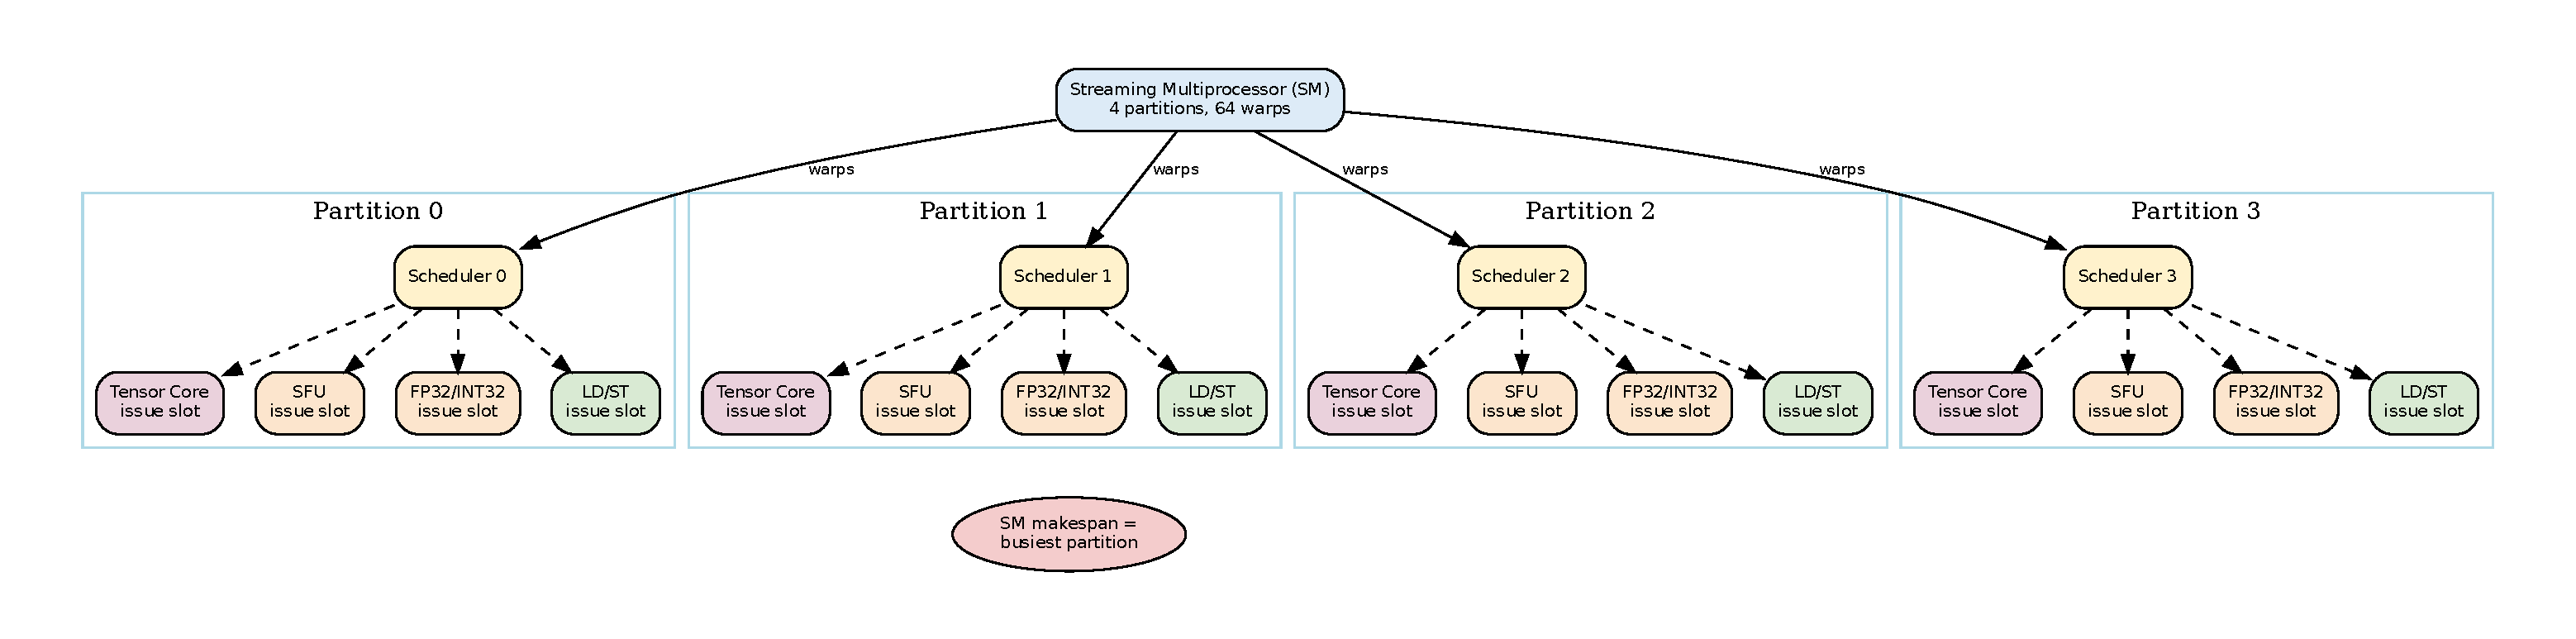
\includegraphics[width=\textwidth]{figures/figure6_subcore_partition.pdf}
\setcounter{figure}{10}
\caption{Sub-core partition scheduling inside one Blackwell SM}
\label{fig:subcore-partition}
\end{figure*}

\end{document}